\documentclass[12pt, a4paper, openany]{book}

\usepackage{fancyhdr}
\usepackage[left=4cm, right=4cm, top=4cm, bottom=4cm]{geometry}
\usepackage[symbol,stable]{footmisc}
\usepackage[utf8]{inputenc}
\usepackage[table]{xcolor}
\usepackage{hyperref}
\usepackage{multirow}
\usepackage{amsmath}
\usepackage{amsfonts}
\usepackage{enumitem}
\usepackage{float}
\usepackage{graphicx}
\usepackage{booktabs}
\usepackage{zref-perpage}
\usepackage{makecell}
\usepackage{subcaption}
\usepackage[justification=centering]{caption}
\usepackage{xepersian}

\DeclareMathOperator*{\argmax}{argmax}
\DeclareMathOperator*{\argmin}{argmin}
\zmakeperpage{footnote}
\newcolumntype{L}{>{$}l<{$}} % math-mode version of "l" column type

\newcommand{\coursetitle}{شبکه‌های عصبی پیچشی تکه‌ای}
\newcommand{\doctitle}{کار مطالعاتی شبکه‌های عصبی}
\newcommand{\name}{محمدرضا غفرانی}
\newcommand{\studentno}{400131076}
\newcommand{\todaydate}{\today}
\renewcommand{\bibname}{منابع و مراجع}

\settextfont{XB Kayhan}
\setlatintextfont{Times Newer Roman}

\pagestyle{fancy}
\lhead{\textbf{\doctitle}}
\chead{\name}
\rhead{\todaydate}

\begin{document}

\begin{center}
    \huge
    \textbf{\coursetitle} \\
    \vspace{1cm}
    \LARGE
    \doctitle \\
    \vspace{1cm}
    \large
    \textbf{\name} \\
    \studentno \\
    \todaydate
\end{center}

% suppress the fancy header on the first page only
\thispagestyle{plain}

\renewcommand*{\thefootnote}{\arabic{footnote}}

\tableofcontents

\clearpage

\chapter{مقدمه}
\clearpage
شبکه عصبی پیچشی تکه‌ای\LTRfootnote{Piecewise Convolutional Neural Network(PCNN)} در ابتدا در سال ۲۰۱۵ توسط ژنگ و همکاران در کنفرانس \lr{ACL} ارائه شد
\cite{zeng-etal-2015-distant}. این شبکه با هدف استخراج روابط بین دو موجودیت در متن ارائه شد. در سال‌های بعد
هم «استخراج رابطه بین موجودیت‌ها» هدف بیشتر  پژوهش‌هایی بود که از این شبکه عصبی استفاده کردند.

با توجه تنیدگی شبکه عصبی پیچشی تکه‌ای و استخراج رابطه نیاز است تا توضیحاتی در رابطه با
شیوه استخراج رابطه بین موجودیت‌ها در متن داده شود.
در استخراج رابطه موجودیت‌ها از روی جمله تلاش می‌شود با داشتن موجودیت‌ها و متن جمله،
رابطه‌ای که جمله بین آن‌ موجودیت‌ها بیان می‌کند، استخراج شود. برای روشن شدن مطلب جمله «حافظ در شیراز درگذشت.» را
در نظر بگیرید.
این جمله شامل دو موجودیت «حافظ» و «شیراز» بوده و رابطه بیان شده توسط این جمله برای این دو موجودیت «محل فوت» است.
هدف این پژوهش‌ها نیز استخراج رابطه «محل فوت» از روی متن جمله و موجودیت‌های آن است.

گرچه استخراج رابطه از متن در نگاه اول ساده به نظر می‌رسد اما این پژوهش‌ها با چالش‌هایی نیز مواجهند. در مثال قبلی جمله رابطه «محل فوت» را بین دو موجودیت
«حافظ» و «شیراز» بیان می‌کرد اما جمله «حافظ در شیراز متولد شد» رابطه «محل تولد» را بین دو موجودیت بیان می‌کند.
همان‌طور که می‌بینید با اندکی تغییر در جمله معنای جمله کاملا می‌تواند متفاوت شود و رابطه دیگری را بین موجودیت‌ها بیان کند.

برای فراهم کردن داده‌های آموزشی برای استخراج رابطه در گذشته از روش‌های بانظارت استفاده می‌شد. اما با توجه به سرآیند زیاد این
روش‌ها مینتز در سال ۲۰۰۹ ایده نظارت‌ازراه‌دور را برای جمع‌آوری داده برای وظیفه استخراج رابطه از روی جمله را
مطرح کرد \cite{mintz-etal-2009-distant}. در این ایده از یک پایگاه دانش که شامل موجودیت‌ها و رابطه بین آن‌ها بود
برای جمع‌آوری داده‌های آموزشی از سطح وب استفاده می‌شود. بدین طریق که هر جمله‌ای که شامل هر دو موجودیت بود به عنوان
نمونه‌ای از رابطه‌ی بیان شده بین دو جمله در نظر گرفته می‌شود. البته همان‌طور که مشخص است این ایده ممکن است جملاتی را نیز
که رابطه دیگری را بیان می‌کنند را به عنوان یک نمونه آموزشی برای رابطه مدنظر جمع‌آوری کند، مثلا این ایده هر دو مثال
ارائه شده در بالا را به عنوان «محل فوت» یا «محل زندگی» در نظر می‌گیرد.
اما از آن جا که حجم داده‌های آموزشی جمع‌آوری شده در این حالت
بسیار زیاد است در مصالحه بین حجم داده برچسب خورده و درستی برچسب‌ها این روش بهتر عمل می‌کند.

حال که زمینه پژوهشی استخراج رابطه از متن بررسی شد، تمرکز خود را روی شبکه عصبی \lr{PCNN} و تلاش‌هایی که برای
بهبود آن انجام شده است می‌دهیم. در ابتدا شیوه عمل شبکه عصبی پیچشی تکه‌ای را مورد بررسی قرار می‌دهیم.

\begin{figure}[h]
    \centering
    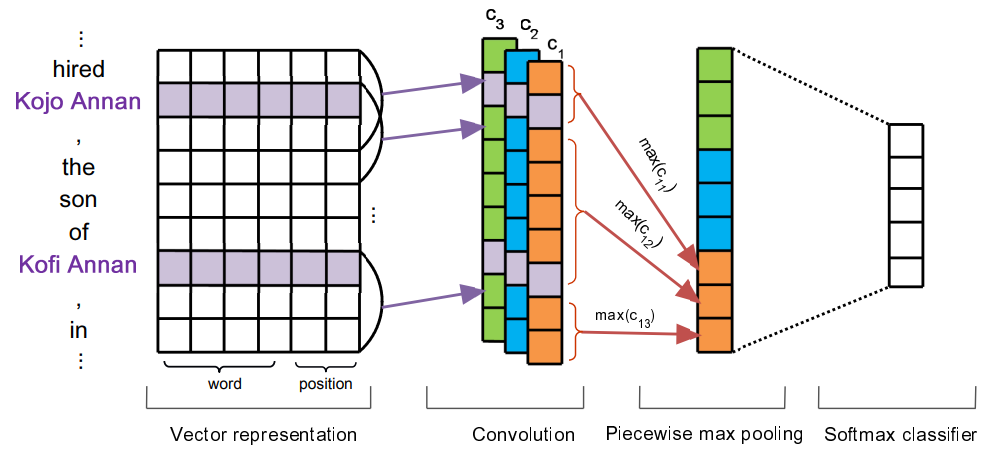
\includegraphics[width=0.8\linewidth]{images/pcnn.png}
    \caption{شبکه عصبی پیچشی تکه‌ای}
    \label{pcnn_architecture}
\end{figure}

در شکل \ref{pcnn_architecture} ساختار شبکه عصبی پیچشی تکه‌ای مشاهده می‌شود. با ورود نمایش برداری کلمات به لایه‌های
کانوولوشنی، این لایه‌ها به صورت سطری روی نمایش برداری پیمایش کرده و ویژگی‌های جمله را استخراج می‌کنند. در ادامه
هر بردار ویژگی استخراج شده توسط لایه کانوولوشنی به سه قسمت تقسیم می‌شود: قسمت قبل از موجودیت اول، قسمت مابین
موجودیت اول و دوم و قسمت بعد از موجودیت دوم. بیشینه هر یک از این قسمت‌ها محاسبه شده و به صورت یک بردار سه‌تایی
در می‌آید. بردار نهایی بازنمایی جمله با ترکیب بردار‌های سه‌تایی متناظر هر یک از لایه‌های کانوولوشنی حاصل می‌شود. در قدم
بعد از این بازنمایی برای کاربرد مدنظر استفاده می‌شود. به عبارتی شبکه \lr{PCNN} یک شبکه کدگذار است که با دریافت یک بازنمایی
با طول متغیر آن را به یک بازنمایی با طول ثابت نگاشت می‌کند. استخراج ویژگی‌های خوب به همراه ارائه بردار با طول ثابت
برای بازنمایی‌های با طول متغیر باعث محبوبیت شبکه‌های عصبی تکه‌ای شده است.

برای بهبود این شبکه‌های عصبی راهکار‌های مختلفی ارائه شده است. یکی از راهکار‌ها مدل ارائه شده توسط پنگ و همکاران
\cite{dilated} است. آن‌ها پیشنهاد کردند برای آن‌ که شبکه عصبی \lr{PCNN} بتواند وابستگی‌های با فاصله زیاد را در جمله
بهتر بازنمایی کند، به جای استفاده از کانوولوشن‌های پیوسته از کانوولوشن‌های دراز\LTRfootnote{dilated} استفاده شود. این لایه‌های
کانوولوشن به جای آن که خروجی را از روی بردار‌های نزدیک به هم محاسبه کند از بردار‌های با فاصله مکانی مشخص
استفاده می‌کند.

شیوه دیگری که برای بهبود این شبکه‌ها استفاده شده است، ترکیب شبکه‌های عصبی بازگشتی با این شبکه‌هاست. این ایده اولین
بار توسط یان و هو \cite{lstm-pcnn} ارائه شد. بازنمایی ارائه شده توسط شبکه عصبی \lr{PCNN} برای هر بخش بازنمایی
مستقلی را ارائه می‌دهد، بنابراین آن‌ها قصد داشتند با عبور بازنمایی تولید شده از
شبکه عصبی حافظه کوتاه‌مدت بلند\LTRfootnote{Long short-term memory} از این استقلال بکاهند.

اما بیشتر پژوهش‌ها تلاش کرده‌اند عملکرد شبکه‌های پیچشی تکه‌ای را با ارائه بازنمایی بهتر از ورودی‌ها بهبود
ببخشند. اکثر این پژوهش‌ها تلاش دارند که با وزن‌دهی به اجزای مهم در ورودی بازنمایی بهتری را با استفاده
از شبکه‌های پیچشی تکه‌ای تولید کنند \cite{nguyen-vietnamese}, \cite{agpcnn-xingya},
\cite{RCPNN-haihong}, \cite{Rusnachenko-opinion} \cite{Li2022}, \cite{gated}. تحقیقات دیگر ایده‌های دیگری برای بهبود عملکرد این شبکه
عصبی پیشنهاد کردند. برای مثلا سانگها نام\LTRfootnote{Sangha Nam} و همکاران \cite{nam-etal-2018-distant} تلاش کردند
بازنمایی بهتری را در ورودی شبکه‌های عصبی پیچشی تکه‌ای برای کلماتی که چندمعنا دارند ارائه دهند. روش پیشنهادی
آن‌ها برای این کار استفاده از یک ماژول ابهام‌زدایی از کلمات بود. در پژوهش دیگری که در سال ۲۰۱۹ انجام شد
تلاش شد با استفاده سلسله‌مراتبی از مدل \lr{PCNN} نتیجه بهتری کسب شود \cite{diyah-adpcnn}.

بعضی دیگر نیز ایده بیان شده توسط شبکه‌های پیچشی تکه‌ای را به شکل دیگری استفاده کرده‌اند. در شبکه
عصبی پیچشی تکه‌ای ابتدا کانوولوشن روی ورودی اعمال شده و سپس خروجی به چند تکه تقسیم می‌شود
اما در مقاله ارائه شده توسط لیو\LTRfootnote{Liu} و همکاران پیشنهاد شد ابتدا ورودی تکه‌تکه شود
و سپس عمل کانوولوشن روی هر قسمت انجام شود \cite{bert}.

به عنوان سخن آخر می‌خواهیم به کاربرد‌های شبکه عصبی \lr{PCNN} در سایز حوزه‌ها اشاره ‌کنیم.
برای این کار می‌توان از پژوهش‌های انجام شده توسط دو\LTRfootnote{Du} و ژنگ\LTRfootnote{Zhang} نام‌ برد.
هر دو این پژوهش‌ها تلاش کرده‌اند با استفاده از شبکه‌های عصبی پیچشی تکه‌ای به نتایج بهتری در حوزه
تحلیل منظور\LTRfootnote{sentiment analysis} انجام دهد. دو از شبکه \lr{PCNN} به عنوان یک کدگذار
استفاده می‌کند و برای افزایش تعداد نمونه‌های آموزشی از شبکه‌های مولد تقابلی\LTRfootnote{Generative Adversarial Network}
بهره می‌گیرد \cite{sentiment-du}. ژنگ نیز مشابه دو به منظور کدگذاری جملات ورودی از شبکه‌های عصبی پیچشی تکه‌ای استفاده
می‌کند \cite{Zhang2018SentimentCB}.

در بخش‌های بعدی با جزئیات برخی از کار‌هایی که در زمینه شبکه‌های عصبی پیچشی تکه‌ای شاخص هستند، را بررسی خواهیم کرد.
در انتها نیز خلاصه‌ای از مطالب ارائه شده و لیست مراجع استفاده شده را خواهیم داشت.

\chapter{شرح مقالات}
\clearpage

\section{استخراج رابطه با تکنیک نظارت از راه دور با استفاده از دروازه در شبکه عصبی پیچشی تکه‌ای با تاکید بر موجودیت‌ها \cite{gated}}

محتوای جمله و به خصوص موجودیت‌ها تاثیر زیادی در معنای برداشت شده از جمله و کلمه دارند. هایخو ون\LTRfootnote{Haixu Wen}، شین‌هوآ ژو\LTRfootnote{Xinhua Zhu}،
لانفانگ ژنگ\LTRfootnote{Lanfang Zhang} و فی لی\LTRfootnote{Fei Li} تلاش کردند با استفاده از مکانیزم توجه به خود\LTRfootnote{self attension}
بهتر بتوانند محتوای جمله را در معنای کلمه دخیل کنند. آن‌ها برای انجام این کار از شبکه عصبی پیچشی تکه‌ای
و مکانیزم دروازه\LTRfootnote{gate} استفاده کردند.

\begin{figure}[h]
    \centering
    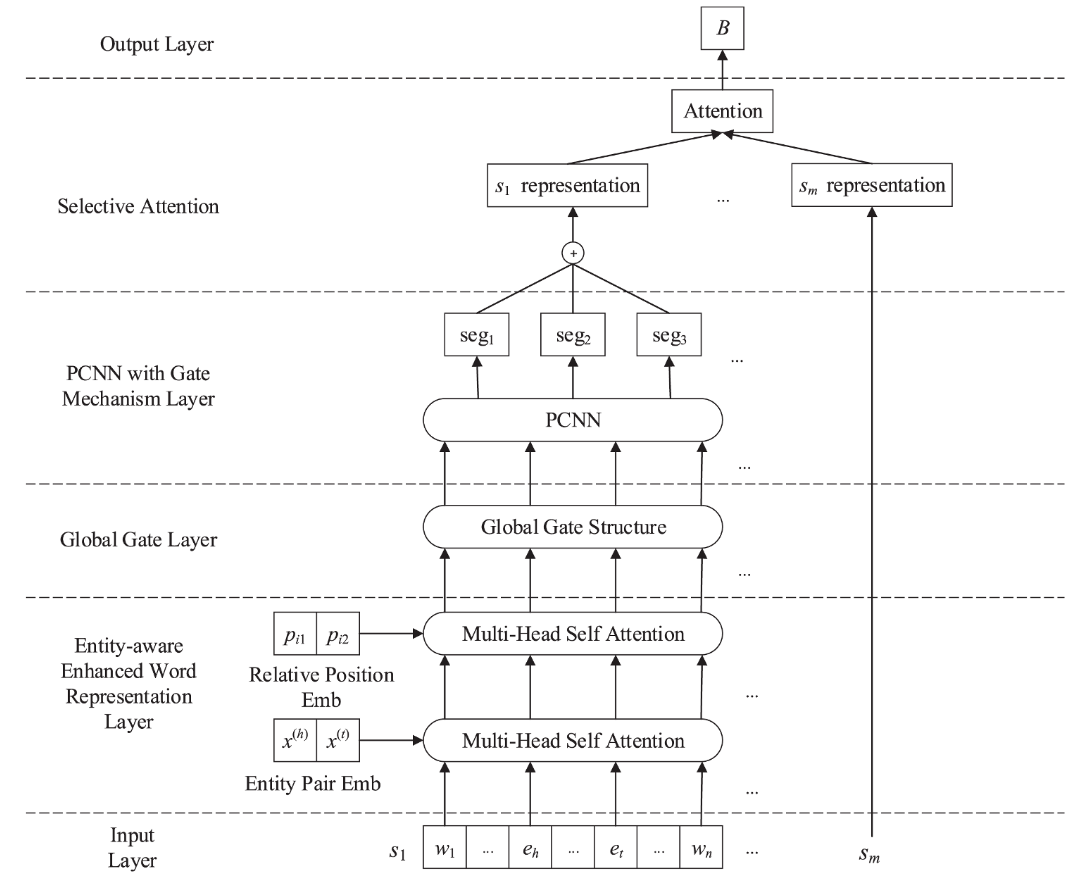
\includegraphics[scale=0.22]{images/gated/architecture.png}
    \caption{معماری شبکه مقاله استخراج رابطه با تکنیک نظارت از راه دور با استفاده از دروازه در شبکه عصبی پیچشی تکه‌ای با تاکید بر موجودیت‌ها}
    \label{gated}
\end{figure}

شکل \ref{gated} خلاصه کار انجام شده توسط ون و همکاران را نشان می‌دهد. در این شبکه ابتدا هر کلمه با استفاده از
مدل \lr{word2vec} به بردار تبدیل می‌شود. در قدم بعدی ترکیب بردار موجودیت‌ها با بردار کلمه
به لایه توجه به خود داده می‌شود تا بازنمایی بهتری برای کلمه با تاکید بر بازنمایی موجودیت‌ها تولید شود. به عبارتی اگر بردار کلمه $i$ام را با $x_i$ و بردار موجودیت اول
را با $e^{h}$ و بردار موجودیت دوم را با $e^{t}$ نمایش دهیم، در این صورت بردار ورودی به لایه توجه به خود برابر خواهد
بود با

\begin{eqnarray}
    [x_i, e^{h}, e^{t}]
\end{eqnarray}

فرض کنیم خروجی لایه توجه به خود در قدم قبلی بردار $x^{h}_i$ باشد. برای پررنگ‌‌‌تر کردن همبستگی بین هر کلمه و
موجودیت‌، بردار $x^{h}_i$ با فاصله مکانی نسبی کلمه تا هر یک از موجودیت‌ها، که آن را با $p_{i,1}$ و
$p_{i,2}$ نشان می‌دهند، ترکیب شده و حاصل مجددا به لایه توجه به خود داده می‌شود. البته این لایه توجه به خود
متفاوت از لایه توجه به خود توضیح داده شده در پاراگراف قبلی است. به عبارتی ورودی لایه توجه به
خود در این حالت برابر خواهد بود با

\begin{eqnarray}
    [x^{h}_i, p_{i,1}, p_{i,2}]
\end{eqnarray}

خروجی قسمت قبل برای هر کلمه را با علامت $x^{ep}_i$ نمایش می‌دهیم. در گام بعدی بردار حاصل شده به لایه دروازه سراسری\LTRfootnote{global gate}
داده می‌شود. ساختار این بخش در شکل \ref{gate_structure} مشاهده می‌شود. در لایه دروازه سراسری ابتدا بردار میانگین یک جمله بر اساس
بردار‌های $x^{ep}_i$ محاسبه می‌شود. برای محاسبه میزان همبستگی بردار میانگین با هر یک از بردار‌های کلمات، حاصل ضرب نقطه‌ای
بین بردار میانگین و بردار کلمه ($x^{ep}_i$) محاسبه می‌شود. در ادامه بردار حاصل شده از حاصل‌ضرب نقطه‌ای با عبور از یک لایه
متراکم حالت ضریب به خود پیدا می‌کند. بردار‌های بازنمایی نهایی با ضرب این مقادیر ضریب در هر یک از بردار‌ها محاسبه می‌شود.
به بیان ریاضی

\begin{eqnarray}
    \bar{x} & = & \frac{1}{n} \sum_{i}^{n} x^{ep}_i \\
    g_i & = & \sigma(W^g (x^{ep}_i \odot \bar{x}) + b^g) \\
    x^{g}_i & = & x^{ep}_i \odot g_i
\end{eqnarray}

\begin{figure}[h]
    \centering
    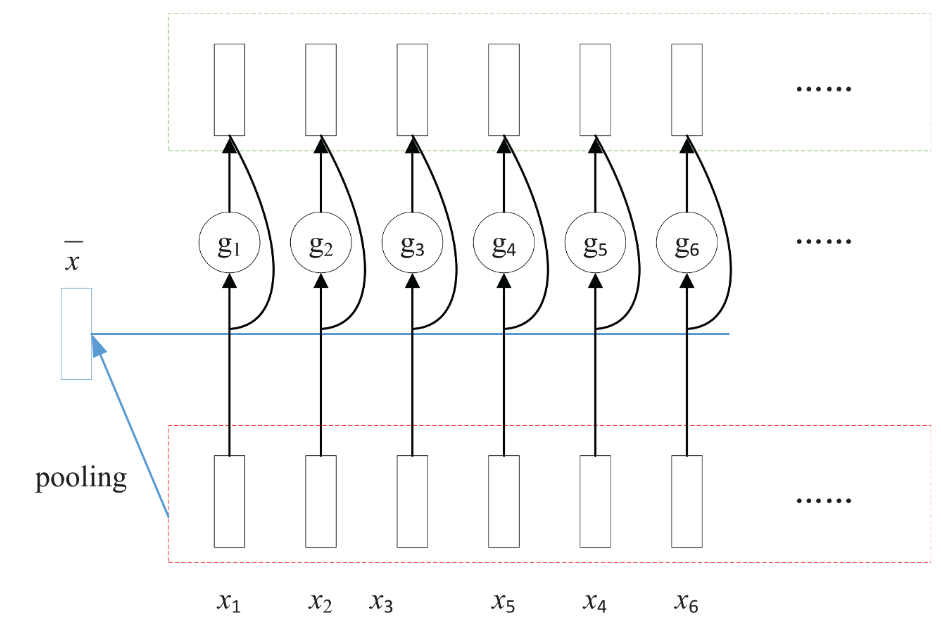
\includegraphics[scale=0.2]{images/gated/gate.png}
    \caption{ساختار قسمت دروازه سراسری}
    \label{gate_structure}
\end{figure}

بردار‌های حاصل شده از لایه دروازه سراسری ($x^{g}_i$) به شبکه \lr{PCNN} داده می‌شود. شبکه \lr{PCNN}
برای سه قسمت جمله بازنمایی متفاوتی را ارائه
می‌کند. این بازنمایی‌ها در ادامه مشابه دروازه سراسری از یک لایه متراکم عبور داده شده و وزن‌های حاصل شده در آن‌ها ضرب می‌شود.
به عبارت ریاضی اگر فرض کنیم خروجی شبکه \lr{PCNN} برابر $[q_{i,1}, q_{i,2}, q_{i,3}]$ باشد، در این صورت خواهیم داشت:

\begin{eqnarray}
    g_{i, seg} & = & \sigma(W^sq_{i,seg} + b^s) \\
    P_{i,seg} & = & g_{i,seg} \odot q_{i,seg} \\
    s^{i}  & = & \tanh([P_{i,1}; P_{i,2}, P_{i,3}])
\end{eqnarray}

بردار $s$ بردار بازنمایی نهایی از یک جمله در این روش است. در این مقاله برای نادیده گرفتن جملات نویزی از وزن‌دهی
جملات یک دسته استفاده می‌شود. بیان ریاضی این قسمت به صورت زیر انجام می‌شود.

\begin{eqnarray}
    B = \sum_{i} \alpha_i s_i \\
    \alpha_i = \frac{\exp(s_iAv_r)}{\sum_{j} \exp(s_jAv_r)}
\end{eqnarray}

بردار $B$ برای آموزش مدل و تعیین برچسب نمونه در هنگام آزمون استفاده می‌شود.



\clearpage
\section{استخراج رابطه با روش نظارت از راه دور با استفاده از شبکه‌های عصبی تکه‌ای با توجه مکانی و توجه به دسته‌های مشابه\cite{Li2022}}

در این مقاله برای بهبود استخراج روابط از جمله‌ها از دو شبکه مجزا استفاده شده است. یکی از این شبکه‌ها در
سطح جمله عمل کرده و دیگری وظیفه تعیین یافتن ویژگی بین جملات یک دسته است. شبکه عصبی توجه مکانی از
مدل \lr{PCNN} برای کدگذاری جملات استفاده کرده و برای ارائه کدگذاری بهتر روش جدیدی را برای توجه به
مکان قرارگیری کلمات پیشنهاد می‌دهد. روش دوم نیز برای رفع استخراج ویژگی‌ از دسته‌هایی که تعداد جملات اندکی دارند
ارائه شده است. در ادامه با جزئیات بیشتر با ساختار هر کدام از این شبکه‌ها آشنا می‌شویم.

\subsection{شبکه عصبی توجه مکانی}

همان‌طور که بیان شد هدف از شبکه عصبی اول ایجاد یک بازنمایی بهتر برای جمله است و برای ایجاد این بازنمایی از
شبکه \lr{PCNN} استفاده می‌شود. برای آن‌ که \lr{PCNN} بتواند بازنمایی دقیق‌تری را ارائه دهد پیشنهاد شده است
که به کلماتی که به موجودیت‌های جمله نزدیک‌تر هستند اهمیت بیشتری داده شود. شمای کلی این شبکه در شکل
\ref{pos_attension} آورده شده است.

شیوه انجام این وزن‌دهی به این صورت است که ابتدا فاصله هر کلمه تا هر یک از موجودیت‌ها محاسبه می‌شود.
با انجام این کار برای هر کلمه دو عدد $d_1$ و $d_2$ به دست می‌آید که $d_1$ فاصله کلمه تا موجودیت اول و $d_2$
فاصله کلمه تا موجودیت دوم است. حال این فاصله‌ها در فرمول تابع چگالی احتمال گاوس با $\mu=0, \sigma=0.5$ قرار داده
می‌شود تا مقادیر کوچک‌تر به اعداد بزرگ‌تر و مقادیر بزرگ‌تر به اعداد کوچک‌تری تبدیل شوند. با این تبدیل مقدار $d_1$ به عدد $G_1$
و عدد $d_2$ به $G_2$ تبدیل می‌شود.

در قدم بعدی برای هر کلمه مقدار $G_1 + G_2$ را محاسبه کرده و حاصل را به تابع \lr{softmax} می‌دهند.
این تابع هر یک از مقادیر را به بازه $[0,1)$ نگاشت می‌کند. از این مقادیر برای وزن‌دهی بازنمایی کلمات
استفاده می‌شود. بردار‌های وزن‌دهی شده برای استخراج ویژگی‌های بیشتر به شبکه \lr{PCNN} داده می‌شود.

\begin{figure}[h]
    \centering
    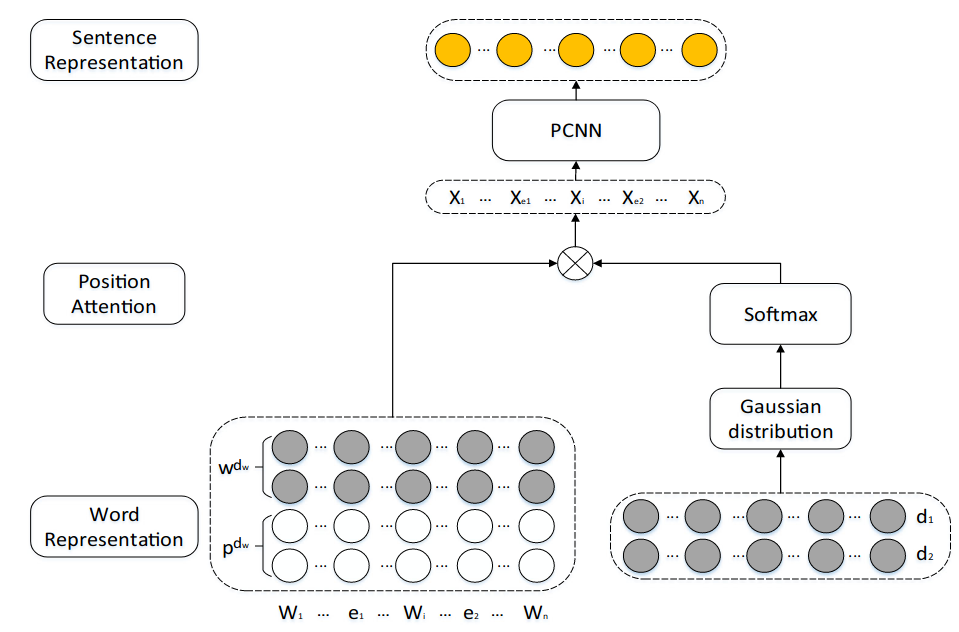
\includegraphics[width=0.8\linewidth]{images/pos_attension/pos_attension.png}
    \caption{مدل بازنمایی جمله}
    \label{pos_attension}
\end{figure}

\subsection{شبکه توجه به دسته‌های با ویژگی‌های مشابه}

مجموعه داده‌ای که برای این پژوهش استفاده شده است، شامل ۵۳ رابطه مختلف است. اما بیشتر برای بیشتر این روابط
تنها یک نمونه وجود دارد. مشخص است که برای چنین دسته‌هایی شبکه قادر نخواهد بود ویژگی‌های مناسبی استخراج کند.
روشی که در این پژوهش ارائه شده است ادغام ویژگی‌های مشابه از دسته‌های دیگر در این شبکه است.

\begin{figure}[h]
    \centering
    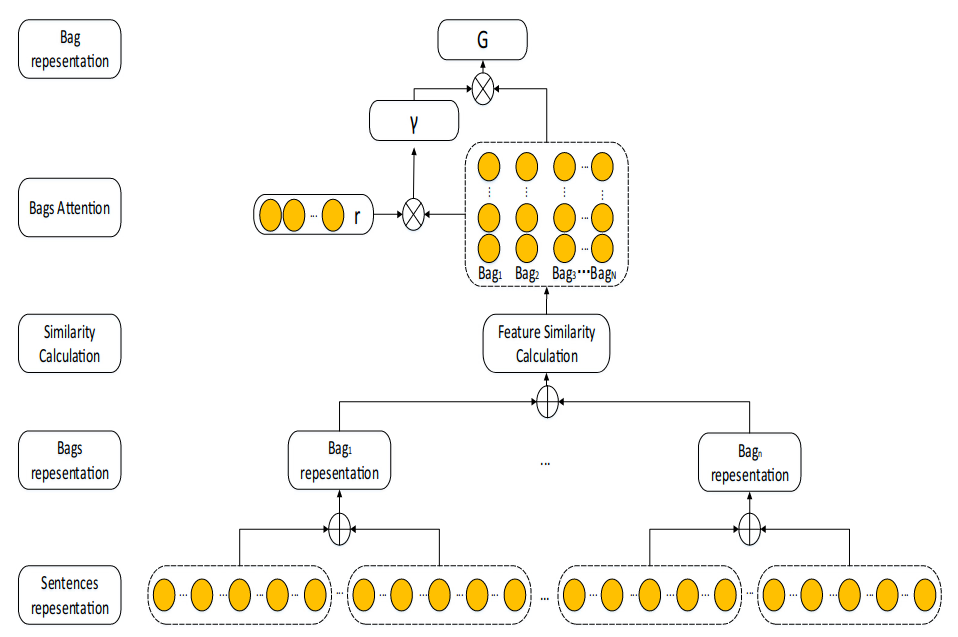
\includegraphics[width=0.8\linewidth]{images/pos_attension/bag_attension.png}
    \caption{ساختار مدل توجه به دسته‌های با ویژگی‌های مشابه}
    \label{bag_attension}
\end{figure}

راهکار ارائه شده به این صورت عمل می‌کند که ابتدا شباهت ویژگی‌های استخراج شده برای دسته فعلی را با ویژگی‌های
تمام دسته‌های دیگر از طریق رابطه‌ی ریاضی زیر محاسبه می‌کنند.

\begin{eqnarray}
    \text{\lr{sim}}(\text{\lr{Bag}}_i, \text{\lr{Bag}}_j) = \text{\lr{Bag}}_i \text{\lr{Bag}}^T_j
\end{eqnarray}

سپس $n$ تا از شبیه‌ترین دسته‌ها انتخاب می‌شود. در قدم بعدی ویژگی‌ها وزن‌دهی شده و بر اساس وزن‌ها
ترکیب می‌شوند. وزن‌های این با استفاده از فرمول زیر استخراج می‌شود.

\begin{eqnarray}
    \gamma_i & = & \frac{\exp(e_i)}{\sum_{k}^{N} \exp(e_k)} \\
    \exp(e_i) & = & \text{\lr{Group}}_i^{j} B r
\end{eqnarray}

در فرمول بالا $B$ یک ماتریس قطری وزن و $r$ یک بازنمایی برداری از رابطه است. پس از محاسبه $\gamma_i$ها ویژگی‌ها
به صورت زیر با هم ترکیب می‌شوند.

\begin{eqnarray}
    G_i = \sum_{i}^{N} \gamma_i \textrm{\lr{Group}}_i^{j}
\end{eqnarray}

برچسب نهایی با استفاده از $G_i$ها تعیین می‌شود.

\clearpage
\section{استخراج رابطه با استفاده از مولد بازنمایی مشترک و شبکه‌های عصبی پیچشی کوتاه‌مدت بلند تکه‌ای \cite{lstm-pcnn}}

در این مقاله که در سال ۲۰۱۸ توسط دانفنگ یان\LTRfootnote{DANFENG YAN} و بو هو\LTRfootnote{BO HU} عرضه شده است،
از یک شبکه عصبی مولد برای ایجاد بازنمایی‌ رابطه استفاده شده است. این شبکه مولد برای ایجاد بازنمایی رابطه از بازنمایی جملات
آن رابطه کمک می‌گیرد. بازنمایی جمله نیز با استفاده از
شبکه‌های عصبی پیچشی کوتاه‌مدت بلند تکه‌ای\LTRfootnote{Piecewise-LSTM Convolutional Neural Network} انجام می‌شود.

\subsection{شبکه‌های عصبی کد‌گذار}

در روش‌های ارائه شده پیش از این مقاله، کدگذاری خام ارائه شده توسط \lr{PCNN} در قسمت‌های بعدی برای تعیین
رابطه بیان شده در جمله استفاده می‌شد. در این مقاله اما پس از کدگذاری جمله توسط شبکه \lr{PCNN} این کدگذاری‌ها مطابق
شکل \ref{pcnn_lstm} به یک شبکه \lr{BiLSTM} داده می‌شود تا ارتباط موجود بین قسمت‌های مختلف جمله در بازنمایی ارائه شده نهایی
تاثیرگذار باشد. کدگذاری تولید شده توسط این شبکه در شبکه‌ مولد که در بخش بعدی خواهیم دید، به کار گرفته می‌شود.

\begin{figure}[h]
    \centering
    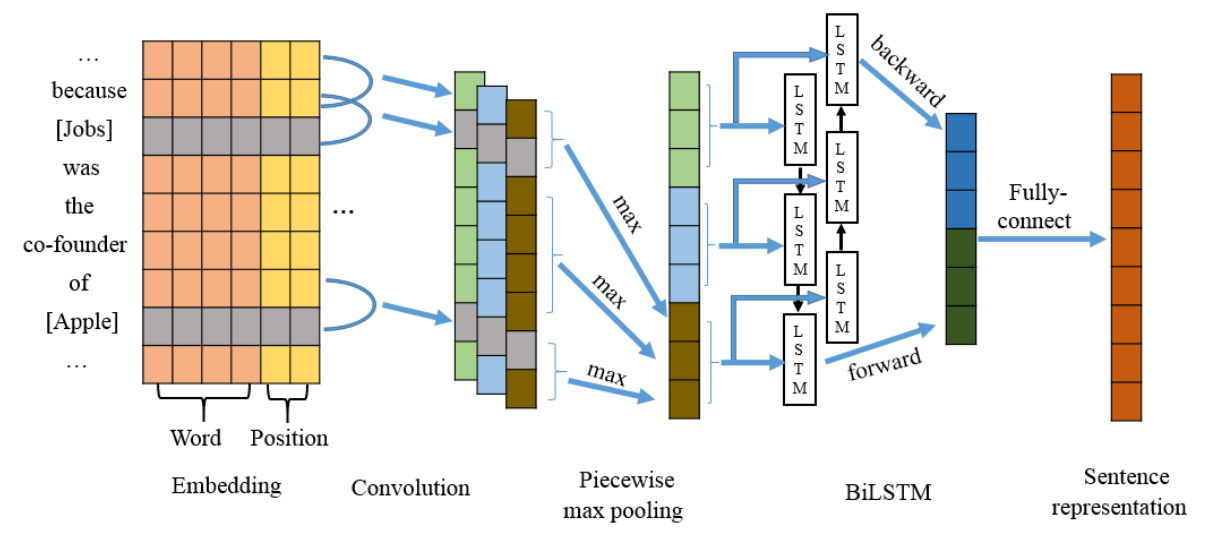
\includegraphics[width=0.8\linewidth]{images/shared/encoder.png}
    \caption{ترکیب شبکه عصبی \lr{PCNN} و \lr{LSTM}}
    \label{pcnn_lstm}
\end{figure}

\subsection{شبکه تولید‌کننده بازنمایی مشترک}

یان و هو شبکه عصبی موجود در شکل \ref{shared_representation_generator_network} را برای ایجاد بازنمایی یک دسته\LTRfootnote{bag}
از کلمات ارائه کردند. آن‌ها بر خلاف پژوهش‌های دیگر به جای آن که از مجموع وزن‌دار بازنمایی هر جمله ($s_{(i,r)}$) برای تولید
بازنمایی مشترک استفاده کنند، پیشنهاد یک مولد برای تولید بازنمایی جملات یک رابطه را مطرح کردند. این مدل مولد برای تولید
بازنمایی رابطه از بازنمایی تولید شده برای جملات متناظر رابطه استفاده می‌کند. برای آموزش این شبکه تابع خطایی نیز
معرفی شده است که ترکیبی از تابع خطای آنتروپی متقابل\LTRfootnote{cross entropy} و میانگین فاصله است.
در ادامه با جزئیات بیشتر این شبکه عصبی و تابع خطای معرفی شده آشنا می‌شویم.

شبکه عصبی مولد برای ایجاد بازنمایی رابطه از بازنمایی‌های جمله‌ که توسط مدل کدگذار \lr{PCNN} تولید شده استفاده می‌کند.
بازنمایی جمله ارائه شده توسط شبکه \lr{PCNN} به شبکه عصبی دولایه داده می‌شود. شبکه عصبی دولایه بازنمایی جمله $i$ام در رابطه
$r$ام را از فضای $s_{(i,r)}$ به فضای $g_{(i,r)}$ می‌برد. هدف از این تبدیل ایجاد یک بازنمایی بهتر با تاکید بیشتر روی معنا از بازنمایی
جمله است. در مدل پیشنهادی آن‌ها برای هر رابطه شبکه مولد جداگانه‌ای در نظر گرفته شده است که از شبکه مولد دیگر
مستقل است.

\begin{figure}[h]
    \centering
    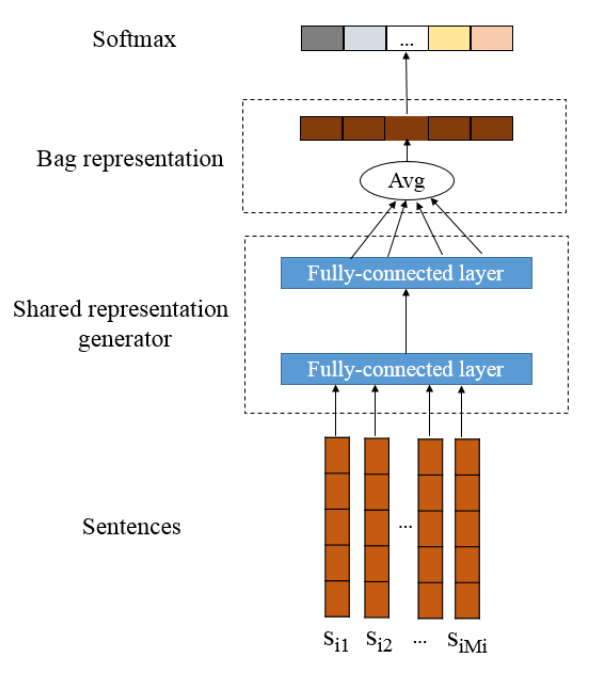
\includegraphics[scale=0.4]{images/shared/shared_repre.png}
    \caption{شبکه عصبی تولید‌کننده بازنمایی مشترک}
    \label{shared_representation_generator_network}
\end{figure}

پس از ایجاد بردار‌های $g_{(i,r)}$، میانگین بدون وزن این بردار‌ها محاسبه می‌شود. بردار حاصل شده $G_{r}$
را بردار بازنمایی آن رابطه می‌نامند.

$$G_{r} = \frac{1}{M} \sum_{i=1}^{M} g_{(i,r)}$$

از آن‌جا که آموزش مدل روی نمونه‌ها به صورت دسته‌ای بوده است، بنابراین در هنگام آزمایش مدل داده‌ها به صورت
دسته‌ای به مدل مولد داده شده و رابطه کلی بیان شده توسط آن‌ دسته با استفاده از یک لایه بیشینه‌گیری نرم\LTRfootnote{softmax}
مشخص می‌شود.

حال که جزئیات شبکه مولد بیان شد، جزئیات تابع خطای متناظر آن تشریح می‌شود. تابع خطای این شبکه دو هدف را دنبال می‌کند:

\begin{enumerate}
    \item بازنمایی ارائه شده برای یک رابطه تا جای امکان دور از بازنمایی رابطه‌های دیگر باشد.
    \item بازنمایی ارائه شده تا جای امکان مشابه بازنمایی ارائه شده برای هر جمله آن رابطه باشد.
\end{enumerate}

برای رسیدن به هدف اول، از تابع خطای آنتروپی متقابل استفاده می‌شود. بدین ترتیب که انتظار می‌رود لایه بیشینه‌گیری‌ نرم
بتواند برچسب دسته را به درستی تعیین کند. به عبارت ریاضی حاصل عبارت زیر باید بیشینه شود.

\begin{eqnarray}
    J_1(\theta) = \sum_{i=1}^{T} \log p(r_i|G_i,\theta)
\end{eqnarray}

برای رسیدن به هدف دوم نیاز است که فاصله بازنمایی تولید شده از هر جمله متناظر آن رابطه کمینه باشد. برای رسیدن
به این هدف تابع خطای $J_2(\theta)$ به صورت زیر محاسبه می‌شود.

\begin{eqnarray}
    J_2(\theta) & = & \frac{1}{T} \sum_{i=1}^{T} (\frac{1}{M_i} \sum_{j=1}^{M_i} (g_{(j,i)} - c_i)^2) \\
    c_i & = & \frac{1}{M_i} \sum_{j=1}^{M_i} g_{(j,i)}
\end{eqnarray}

نکته عجیبی که در تابع خطای بالا وجود دارد استفاده از بازنمایی $g_{(i,r)}$ به جای $s_{(i,r)}$ است. چرا که
$G_r$ میانگین \textbf{بدون وزن} از $g_{(i,r)}$ است بنابراین محاسبه فاصله آن تا هر یک از $g_{(i,r)}$ به نظر نمی‌رسد که
پارامتری را تحت تاثیر قرار دهد. اما اگر این مقدار از روی $s_{(i,r)}$ از روی محاسبه می‌شد با توجه به این که $g_{(i,r)}$
از یک شبکه عصبی محاسبه می‌شود بنابراین پارامتر‌های این شبکه را تحت تاثیر قرار می‌داد.

در نهایت تابع خطای کل به صورت زیر محاسبه می‌شود.

\begin{eqnarray}
    J(\theta) = J_1(\theta) + \alpha J_2(\theta)
\end{eqnarray}

\clearpage
\section{دسته‌بندی رابطه با بهره‌گیری از مدل \lr{BERT} و کانولوشن‌های تکه‌ای به همراه خطای کسری \cite{bert}}

در سال ۲۰۲۱ لیو\LTRfootnote{Liu} و همکارانش رویکرد متفاوتی را در رابطه با شبکه‌های عصبی پیچشی تکه‌ای در پیش گرفتند.
آن‌ها به جای این که یک کانولوشن را روی شبکه انجام داده و خروجی آن‌ را سه قسمت کنند سه کانولوشن متفاوت را
روی سه قسمت جمله اجرا کردند. با ترکیب خروجی‌های این سه قسمت رابطه‌ای که جمله بیان می‌کند تشخیص داده می‌شود.

\begin{figure}[h]
    \centering
    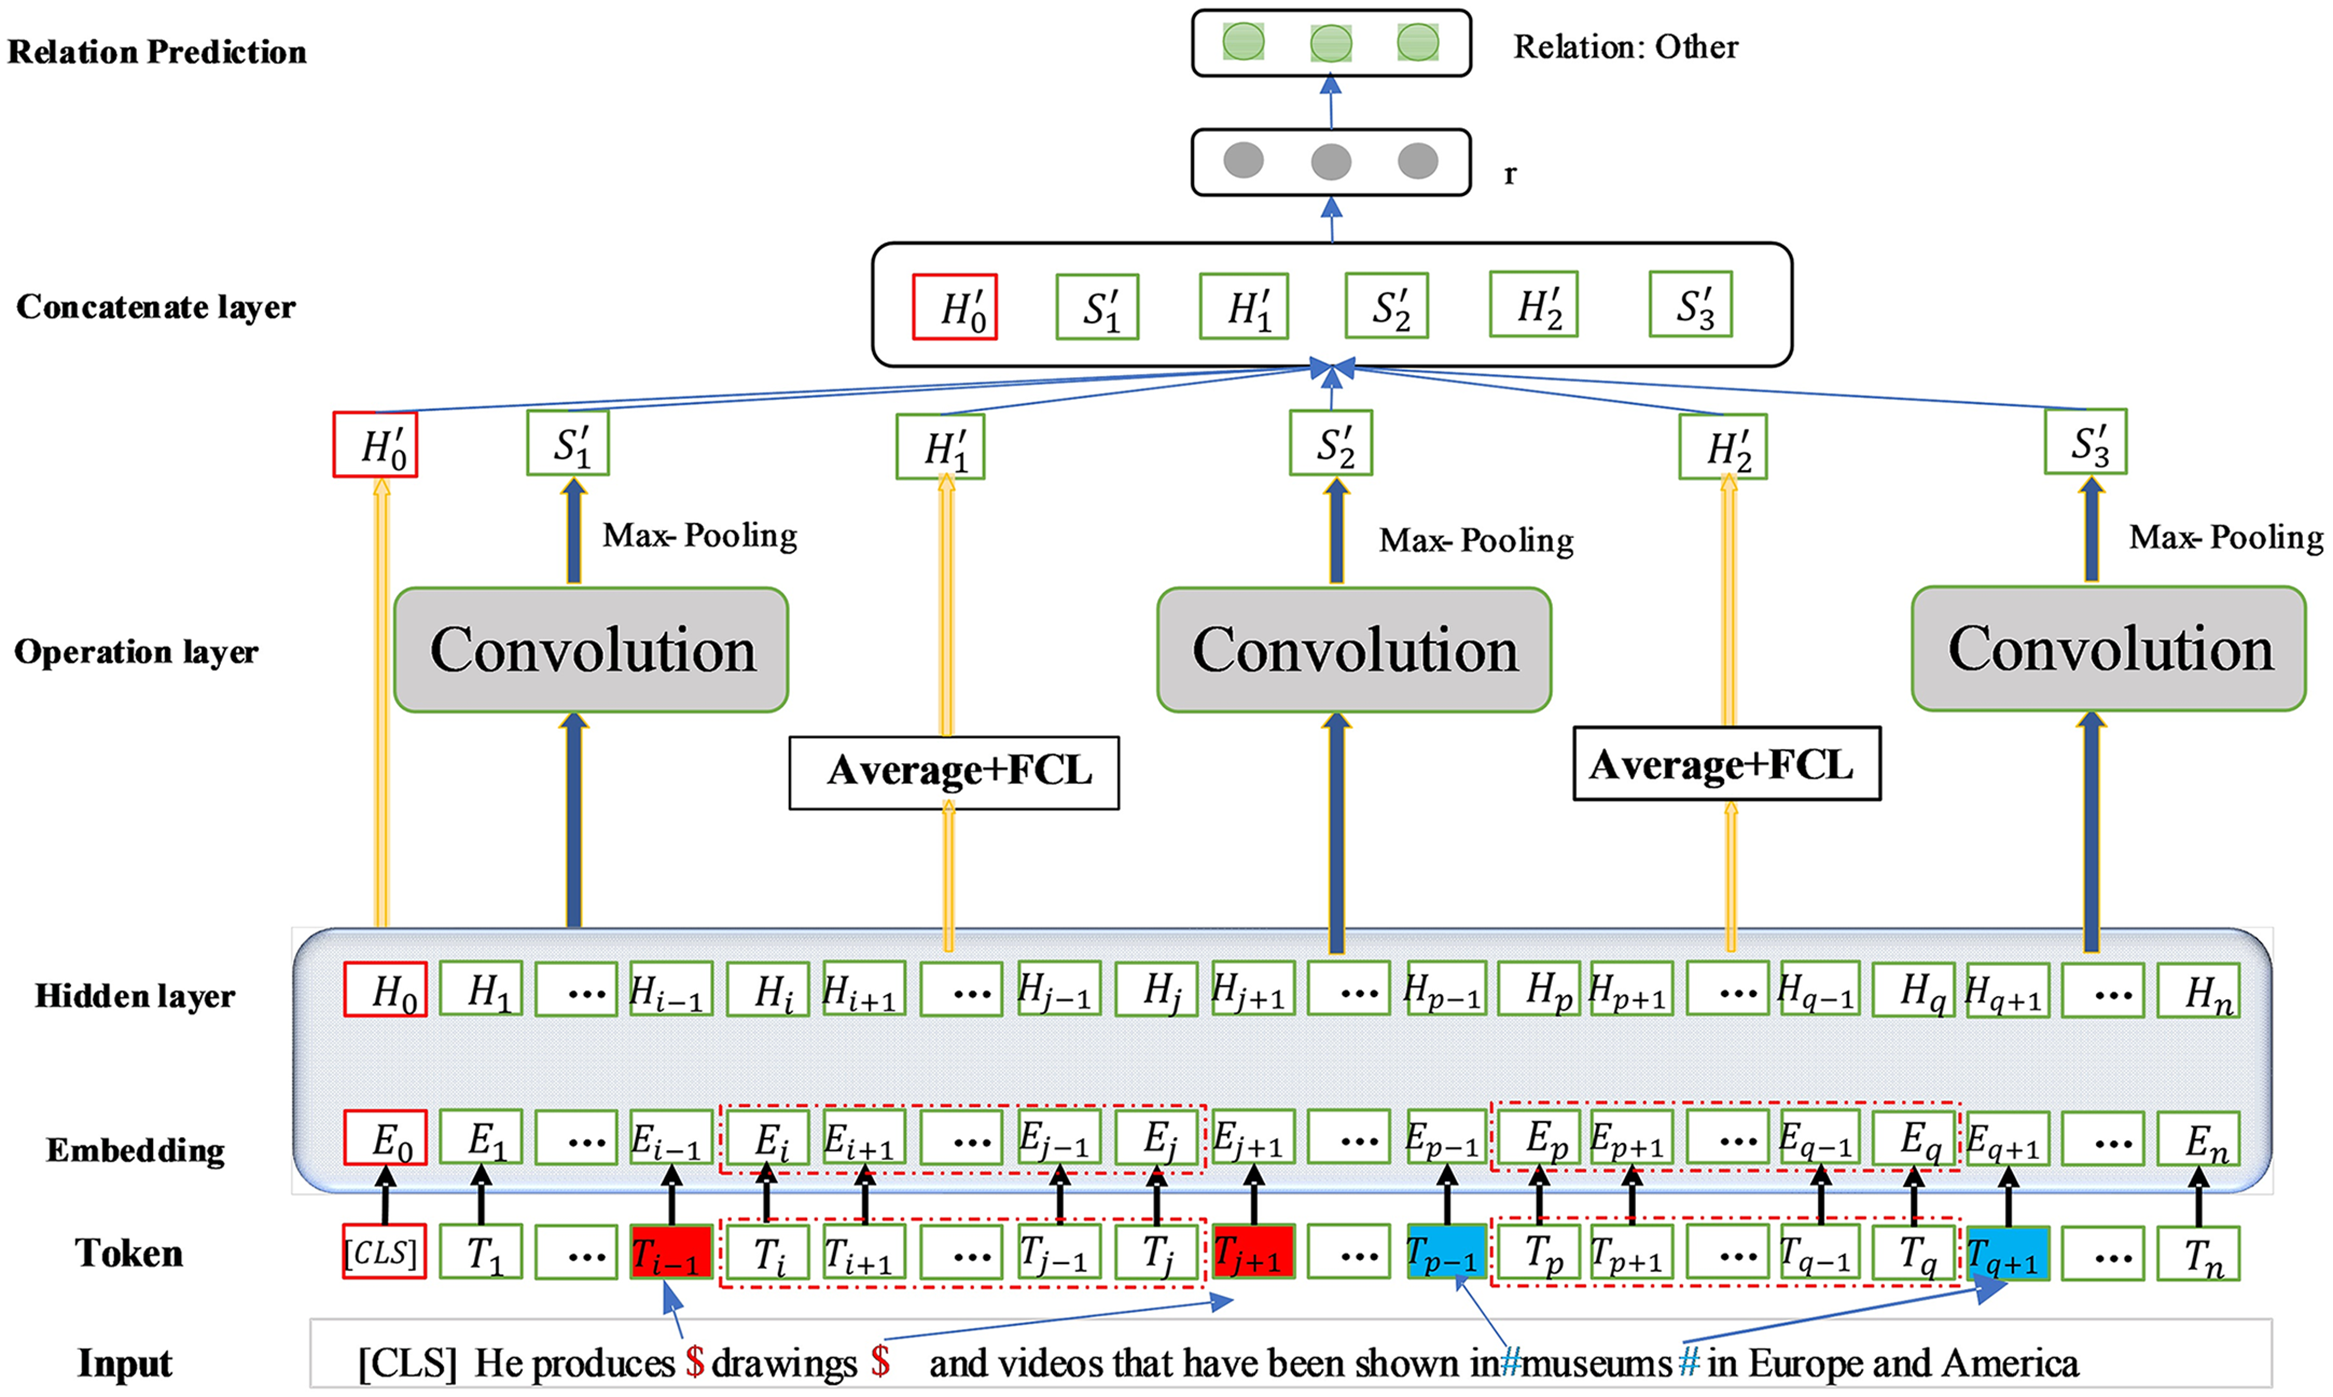
\includegraphics[width=\linewidth]{images/bert/architecture.png}
    \caption{ساختار مدل پیشنهادی}
    \label{article1_architecture}
\end{figure}

مدل پیشنهادی لیو و همکارانش در شکل \ref{article1_architecture} دیده می‌شود. مدل پیشنهادی آن‌ها انتظار دارد موجودیت‌های موجود
در جمله با علامت مخصوصی نظیر $\$$ و $\#$ مشخص شده باشد. با دریافت جمله، توکن‌های \lr{[CLS]} و
\lr{[SEP]} به جمله اضافه شده و جمله به مدل \lr{BERT} داده می‌شود. پس از دریافت بازنمایی کلمات $(E_i)$ از مدل \lr{BERT} هر
بازنمایی از یک لایه \lr{Dense} عبور کرده و بازنمایی دیگری به نام $H_i$ را تولید می‌کند. در این مرحله بازنمایی توکن‌ها
به شش دسته تقسیم شده و برای هر بخش روند متفاوتی طی می‌شود.

\begin{itemize}
    \item \textbf{توکن آغاز جمله \lr{BERT}}: بر روی بازنمایی این توکن عملیات خاصی انجام نشده و مستقیما به خروجی
    منتقل می‌شود.
    \item \textbf{کلمات قبل از موجودیت اول}: بازنمایی متناظر این کلمات $(H_i)$ ها از یک لایه کانولوشن عبور کرده و
    در قدم بعدی \lr{max pooling} گرفته می‌شود. به عبارت ریاضی
    \begin{flalign}
        X_{i:i+h-1} & = H_i \oplus H_{i+1} \oplus H_{i+2} \oplus ... \oplus H_{i+h_1} \\
        c_i & = W * X_{i:i+h-1} + b
    \end{flalign}
    در عبارت بالا منظور از عملگر $\oplus$ عملگر \lr{concatenation} منظور از عملگر $*$ کانولوشن است.
    بنابراین $c_i$ یک عدد بردار در فضای $\mathbb{R}^d$ است. با اعمال این کانولوشن با پنجره $h$
    روی بازنمایی کلمات ماتریس $C$ به شکل زیر تولید می‌شود. ماتریس $C$ در فضای $\mathbb{R}^{(n-h+1) \times d}$
    است.
    \begin{flalign}
        C = \left[ c_1, c_2, ..., c_{n-h+1}\right]
    \end{flalign}
    حال بر روی این ماتریس عملیات \lr{max pooling} انجام می‌شود. هدف از انجام این عملیات علاوه بر کاهش
    ابعاد به فضای $\mathbb{R}^{n-h+1}$، انتخاب مهم‌ترین ویژگی از هر یک از $c_i$هاست.
    \begin{flalign}
        s = \max(C)
    \end{flalign}
    بردار $s$ به مرحله بعدی منتقل می‌شود.
    \item \textbf{موجودیت اول}: از آن جا که ممکن است موجودیت اول خود شامل چند کلمه و در نتیجه دارای بازنمایی چندبعدی باشد بنابراین
    ابتدا میانگین این بازنمایی را پیدا کرده و به عنوان بازنمایی موجودیت اول در نظر می‌گیریم. با عبور این بازنمایی از
    یک لایه \lr{Dense} مقدار $H'_1$ تولید می‌شود. به عبارت ریاضی
    \begin{eqnarray}
        H'_1 = W_1(\tanh(\frac{1}{j-i+1} \sum_{t=i}^{j}{H_t})) + b_1
    \end{eqnarray}
    \item \textbf{کلمات بین دو موجودیت}: برای این کلمات علمیات مشابهی مانند عملیات انجام شده بر روی کلمات
    قبل از موجودیت اول انجام می‌شود.
    \item \textbf{موجودیت دوم}: در این حالت نیز عملیات مشابهی نظیر عملیات انجام شده روی موجودیت اول انجام می‌شود.
    \item \textbf{کلمات بعد از موجودیت دوم}: عملیات انجام شده در این قسمت مشابه عملیات انجام شده روی کلمات
    قبل از موجودیت اول است.
\end{itemize}

پس از استخراج بردار‌های متناظر هر قسمت یعنی $H'_0$، $H'_1$، $H'_2$، $S'_1$، $S'_2$ و $S'_3$ این بردار‌ها با هم
ترکیب شده و به یک لایه \lr{Dense} با تابع فعال‌سازی \lr{softmax} داده می‌شوند.
بیان ریاضی این عملیات به شرح زیر است.

\begin{flalign}
    r = & \; W_r(H'_0 \oplus S'_1 \oplus H'_1 \oplus S'_2 \oplus H'_2 \oplus S'_3) + b_r \\
    \tilde{y} = & \; \sigma(r)
\end{flalign}

در روابط بالا منظور از $\sigma$ تابع \lr{softmax} است. این تابع برای هر دسته یک احتمال نسبت می‌دهد. دسته‌ای که بیشترین
احتمال را داشته باشد به عنوان خروجی نهایی مدل در نظر گرفته می‌شود.

\subsection{تابع خطا}

بیشتر پژوهش‌هایی که در زمینه استخراج رابطه انجام شده‌اند از تابع خطای آنتروپی متقابل\LTRfootnote{cross entropy} که به شرح زیر
تعریف می‌شود برای محاسبه خطای مدل استفاده کرده‌اند. مشکلی که این تابع دارد این است که نسبت به
کلاس‌های با تعداد نمونه زیاد (و در نتیجه آسان بودن یادگیری این کلاس‌ها) بایاس داشته و اعداد
بالایی را برای آن‌ها گزارش می‌دهد.

\begin{flalign}
    J(\theta) = - \sum_{i} y_i \log(p_t) + (1-y_i) \log(1-p_t)
\end{flalign}

برای رفع مشکل این مشکل لیو و همکاران از ایده‌ای که در سال ۲۰۱۷ توسط لین و همکارانش \cite{focal-loss} ارائه شد،
استفاده کرده‌اند. تابع خطای معرفی شده توسط لین تابع خطای کسری\LTRfootnote{focal loss} نامیده شده و به شرح زیر
تعریف می‌شود.

\begin{flalign}
    FL(p_t) = - a_t (1-p_t)^{\gamma} \log(p_t)
\end{flalign}

در این فرمول $\alpha_t$ فاکتور وزن‌دهی نامیده شده و مقداری بین $\left[0,1\right]$ دارد. $\gamma$ نیز پارامتر توجه
نامیده می‌شود. $p_t$ نیز احتمالی است که مدل با آن احتمال درصد اطمینان را گزارش می‌دهد.
برای روشن‌تر شدن مفهوم هر یک از این پارامتر‌ها از یک مثال استفاده می‌کنیم.

فرض کنید دو دسته داریم که فراوانی هر یک از تعداد کل داده‌ها به ترتیب $0.1$ و $0.25$ باشد. همچنین فرض کنید دو مدل
مختلف نیز داریم. مدل اول روی دسته با فراوانی کم‌تر با اطمینان $0.8$ و روی دسته با فراوانی بیشتر با اطمینان $0.85$ درصد
پیش‌بینی انجام می‌دهد. مدل دوم در دسته با فراوانی کم‌تر با اطمینان $0.6$ و در دسته با فراوانی زیاد با اطمینان $0.95$ درصد
پیش‌بینی انجام می‌کند. اگر بخواهیم این عملکرد این دو مدل را با تابع خطای \lr{cross entropy} نسبت به هم بسنجیم،
خواهیم داشت.

\begin{flalign}
    FL(\text{\lr{model}}_1) = & - 0.1 \times (1-0.8)^2 \times \log(0.8) - 0.25 \times (1-0.85)^2 \times \log(0.85) \simeq 0.002 \\
    FL(\text{\lr{model}}_2) = & - 0.1 \times (1-0.6)^2 \times \log(0.6) - 0.25 \times (1-0.95)^2 \times \log(0.95) \simeq 0.008
\end{flalign}

همان‌طور که مشاهده می‌شود تابع خطای کسری برای مدل دوم عدد بزرگتری را گزارش می‌دهد که منطقی است. چرا که مدل دوم در زمانی
که داده بیشتری داشته بهتر و زمانی که با کمبود داده مواجه بوده است عملکرد ضعیفی داشته است. در این مثال مقدار $\gamma=2$
و مقدار $\alpha_t$ را نسبت داده‌های دسته به تعداد کل داده‌ها در نظر گرفتیم. در این مقاله نیز مقدار $\alpha_t$ به همین شکل
انتخاب می‌شود.

حال که با چگونگی رفتار تابع خطا آشنا شدیم، چگونگی اعمال این ایده در تابع آنتروپی متقابل را
مطالعه می‌کنیم. با اعمال این ایده تابع خطای آنتروپی متقابل به شکل زیر در می‌آید.

\begin{flalign}
    J(\theta) = - \sum_{i} \alpha_t y_i (1-p_t)^{\gamma} \log(p_t) + \alpha_t (1-y_i) p_t^{\gamma}\log(1-p_t)
\end{flalign}

این تابع خطا به خوبی دسته‌های با برچسب کم را در نظر می‌گیرد. در این مقاله علاوه بر این کار یک مقدار منظم‌سازی نیز روی
تابع اعمال شده و تابع خطا به شکل زیر حاصل می‌شود.

\begin{flalign}
    J(\theta) = - \sum_{i} \alpha_t y_i (1-p_t)^{\gamma} \log(p_t) + \alpha_t (1-y_i) p_t^{\gamma}\log(1-p_t) + w ||\theta||^2
\end{flalign}

وزن‌های مدل با استفاده از این تابع خطا به روز می‌شود.


\chapter{مجموعه داده}
\clearpage
مقالات بررسی شده از مجموعه داده‌های مختلفی استفاده کرده‌اند که در این جا به صورت
خلاصه جزئیات آن‌ها بررسی می‌شود.

\section{مجموعه داده روزنامه نیویورک تایمز}

مجموعه داده نیویورک تایمز \LTRfootnote{NYT-dataset} در سال 2010 توسط ریدال \cite{nyt-dataset} ارائه شد.
این مجموعه داده که شامل ۵۳ رابطه مختلف است،
یکی از مجموعه داده‌های پرکاربرد در حوزه استخراج رابطه بوده و توسط مقالات مختلف استفاده
شده است. برای ساخت این مجموعه داده از روش نظارت از راه دور استفاده شده و جملات روزنامه نیویورک‌تایمز
با استفاده از پایگاه دانش فری‌بیس\LTRfootnote{freebase} برچسب‌گذاری شده است.
این مجموعه داده شامل ۵۲۲۶۱۱ جمله برای آموزش و ۱۷۲۴۴۸ جمله برای آزمون است.

\section{مجموعه داده \lr{SemEval-2010}}

مجموعه داده \lr{SemEval-2010} نیز در سال ۲۰۱۰ ارائه شده است \cite{hendrickx-etal-2010-semeval}.
این مجموعه داده نسبت به مجموعه داده نیویورک تایمز کوچک‌تر بوده و شامل ۱۹ رابطه مختلف است.
این مجموعه داده شامل 10717 جمله است که از این تعداد 8000 جمله برای آموزش و باقی برای آزمون
استفاده می‌شود.

\section{مجموعه داده \lr{SemEval-2018}}

این مجموعه داده در سال ۲۰۱۸ با برچسب‌گذاری داده‌های گزارش‌ حملات امینتی ارائه شد \cite{phandi-etal-2018-semeval}.
تعداد جملات برچسب‌گذاری شده این مجموعه داده مشابه مجموعه داده \lr{SemEval-2010} بوده اما تعداد
رابطه‌های آن نسبت به مجموعه داده \lr{SemEval-2010} بسیار کم‌تر است. این مجموعه داده شامل
10182 جمله است که از این تعداد ۸۹۱۹ جمله برای آموزش مدل و باقی 1263 جمله برای آزمون استفاده می‌شود.
این مجموعه داده شامل ۴ رابطه مختلف است.

\section{مجموعه داده \lr{UW}}

این مجموعه داده در سال ۲۰۱۶ توسط لیو\cite{liu-etal-2016-effective} ارائه شده است. این مجموعه داده شامل ۵ رابطه
بوده اما تعداد جملاتی که برای هر رابطه ارائه کرده است در اندازه مجموعه داده نیویورک تایمز است. این مجموعه داده دارای
حدود ۵۰۰ هزار جمله برای آموزش و حدود ۳۷۲۴ جمله برای آزمایش مدل است.

\chapter{نتایج}
\clearpage
مقالاتی که در فصل‌های قبل‌تر معرفی شد بیشتر در سطح دسته\LTRfootnote{bag} عمل می‌کنند. بدین معنی که در هنگام آموزش
برای آن که نویز حاصل از برچسب‌زنی با روش نظارت از راه دور را کم کنند، تمامی جملاتی را که برچسب رابطه یکسان دارند
و همچنین شامل دو موجودیت مد نظر هستند به صورت یکجا برای استخراج ویژگی‌ها استفاده می‌کنند.

مقالاتی که بر طبق روش بالا عمل می‌کنند از روش‌های مختلفی ارزیابی می‌شوند. برای ارزیابی این روش‌ها از روشی موسوم به نام
«بسط»\LTRfootnote{hold out} استفاده می‌شود. در این روش نیمی از نمونه جملات متناظر
هر رابطه را به عنوان داده آموزشی و نیم دیگر را به عنوان داده آزمون در نظر می‌گیرند. از معیار‌های مختلفی نظیر
منحنی دقت-بازیابی\LTRfootnote{precision-recall curve}، سطح زیر نمودار\LTRfootnote{area under the curve}
و روشی به نام \lr{P@N} ،برای بررسی عملکرد مدل روی داده‌های آزمون استفاده می‌کنند. علاوه بر این معیار‌ها
گاهی عامل انسانی نیز برای ارزیابی عملکرد مدل استفاده می‌شود.

در مقالاتی که بر اساس تک جمله کار می‌کنند یعنی هم در مرحله آموزش و هم در مرحله آزمون از تک جمله
بهره می‌گیرند از معیار‌هایی نظیر دقت\LTRfootnote{Precision}، بازیابی\LTRfootnote{Recall}
و \lr{F1} برای ارزیابی کار خود استفاده می‌کنند.

در ادامه نتایج مقالات را بر طبق معیار‌های معرفی شده ارائه کرده و مقایسه می‌کنیم.
در این جا برای سادگی، مدل‌های ارائه شده را با نام مخفف انگلیسی آن‌ها اسم می‌بریم.
در ادامه اسم مخفف هر یک از مقالات معرفی می‌شود.

\begin{itemize}
    \item \lr{EA-GPCNN}: شبکه عصبی پیچشی تکه‌ای با تاکید بر موجودیت‌ها
    \item \lr{PCNN-PATT+SBA}: شبکه عصبی پیچشی تکه‌ای با توجه مکانی و توجه به دسته‌های مشابه
    \item \lr{PLSTM-CNN}: شبکه عصبی پیچشی کوتاه‌مدت بلند تکه‌ای
    \item \lr{BERT-PCNN}: شبکه عصبی پیچشی تکه‌ای بر پایه مدل برت\LTRfootnote{BERT}
\end{itemize}

سه مقاله اول در هنگام آموزش بر اساس ویژگی‌هایی که از دسته استخراج کرده‌اند آموزش می‌بینند
در حالی که روش آخر یعنی همواره \lr{BERT-PCNN} در سطح جمله عمل می‌کند. بنابراین سه روش اول را به صورت جدای
از روش آخر بررسی خواهیم کرد.

نمودار دقت-بازیابی برای سه روش \lr{EA-GPCNN}، \lr{PCNN-PATT+SBA} و \lr{PLSTM-CNN} در شکل \ref{recall_precision}
مشاهده می‌شود. همان‌طور که مشاهده می‌شود متاسفانه هیچ یک از مقالات نتیجه خود را با نتیجه مقاله دیگر مقایسه نکرده است،
بنابراین این روش‌ها را صرفا می‌توان از روی شکل ارائه شده با هم مقایسه کرد. بر اساس شکل‌ها عملکرد روش \lr{EA-GPCNN}
از دو روش دیگر بهتر است چرا که بر طبق نمودار به ازای مقادیر یکسان بازیابی نتایج بهتری برای دقت ارائه کرده است.

\begin{figure}[h]
    \begin{subfigure}{0.3\linewidth}
        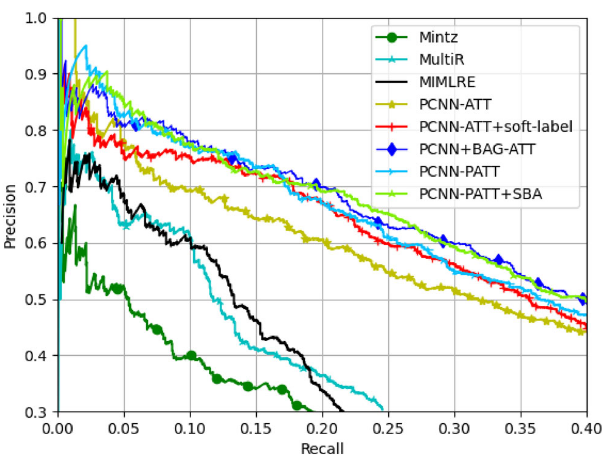
\includegraphics[width=\linewidth]{images/pos_attension/performance.png}
        \caption{عملکرد مدل \lr{PCNN-PATT+SBA}}
    \end{subfigure}
    \begin{subfigure}{0.3\linewidth}
        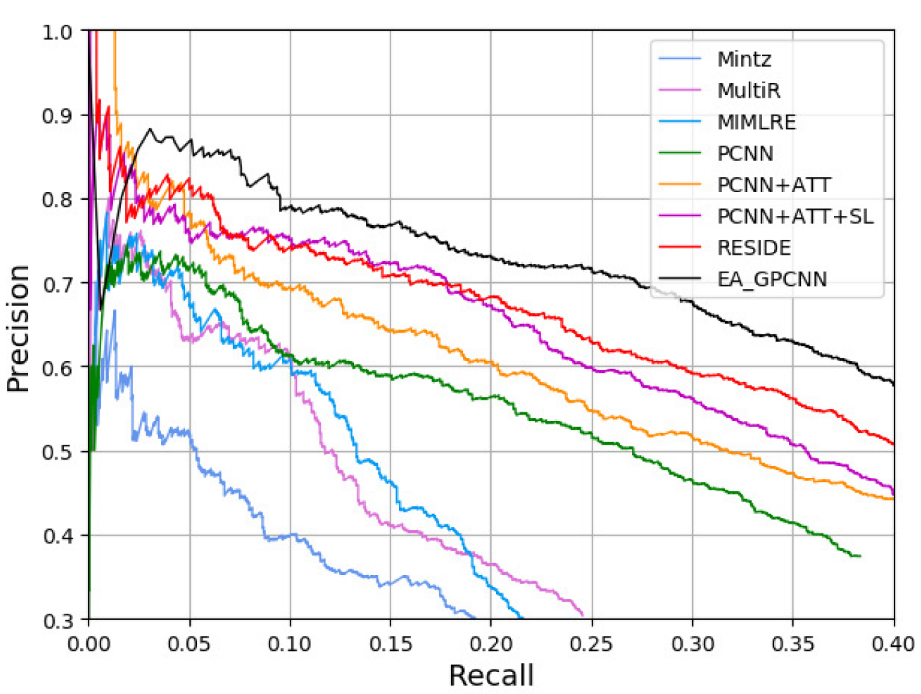
\includegraphics[width=\linewidth]{images/gated/performance.png}
        \caption{عملکرد مدل \lr{EA-GPCNN}}
    \end{subfigure}
    \begin{subfigure}{0.3\linewidth}
        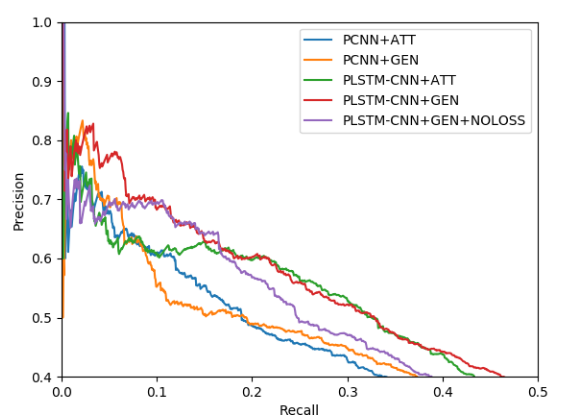
\includegraphics[width=\linewidth]{images/shared/nyt_dataset.png}
        \caption{عملکرد مدل \lr{PLSTM-CNN}}
    \end{subfigure}
    \caption{بررسی عملکرد سه روش \lr{EA-GPCNN}، \lr{PCNN-PATT+SBA} و \lr{PLSTM-CNN} در مجموعه داده نیویورک تایمز}
    \label{recall_precision}
\end{figure}

روش دیگری که این سه مدل را می‌توان بررسی کرد روشی به نام \lr{P@N} است. در این روش دقت عملکرد مدل به ازای
$N$ نمونه آزمون بررسی می‌شود نتایج این بررسی در جدول \ref{pn} مشاهده می‌شود. همان‌طور که مشاهده می‌شود در این معیار
ارزیابی نیز روش \lr{EA-GPCNN} برتر از دو روش دیگر عمل کرده است.

\begin{latin}
\begin{table}[h]
    \centering
    \caption{\rl{بررسی عملکرد سه روش \lr{EA-GPCNN}، \lr{PCNN-PATT+SBA} و \lr{PLSTM-CNN} در مجموعه داده نیویورک تایمز بر معیار \lr{P@N}}}
    \label{pn}
    \begin{tabular}{c|c|c|c|c}
        P@N & 100 & 200 & 300 & mean \\
        \hline
        EA-GCPNN & 91 & 87.5 & 82.0 & 86.8 \\
        PLSTM-CNN & 76.3 & 65.6 & 60.2 & 67.4 \\
        PCNN-PATT+SBA & 86 & 81 & 76.7 & 81.2
    \end{tabular}
\end{table}
\end{latin}

بر طبق معیار‌های ارزیابی بالا بهترین روش \lr{EA-GCPNN} است. این روش بازنمایی هر کلمه را بر اساس فاصله آن از موجودیت
وزن‌دهی می‌کند. در مقام بعدی روش \lr{PCNN-PATT+SBA} است که از مکانیزم توجه استفاده کرده و
دسته‌های با ویژگی‌های مشابه را در هم ادغام می‌کرد. در نهایت روش \lr{PLSTM-CNN} است که از شبکه عصبی \lr{LSTM}
برای بهبود کدگذاری ارائه شده توسط \lr{PCNN} بهره می‌برد. این نتایج نشان از اهمیت دخیل کردن بازنمایی موجودیت در
بازنمایی سایر کلمات دارد چرا که روش‌هایی که به این بخش بیشتر اهمیت داده‌اند نتایج بهتری گرفته‌اند.

تا به این جا نتایج عملکرد سه مدل \lr{EA-GPCNN}، \lr{PCNN-PATT+SBA} و \lr{PLSTM-CNN} را با هم مقایسه کردیم.
در ادامه می‌خواهیم نتایج عملکرد مدل \lr{BERT-PCNN} که رویکرد متفاوتی نسبت به روش‌های نامبرده دارد را
بررسی می‌کنیم.

ارزیابی روش \lr{BERT-PCNN} بر روی مجموعه داده‌های \lr{SemEval-2010} و \lr{SemEval-2018} انجام شده است.
این مدل می‌تواند روی مجموعه داده \lr{SemEval-2010} به نتیجه $89.95$ درصد روی معیار \lr{F1} برسد. عملکرد مدل روی مجموعه داده
\lr{SemEval-2018} از این هم بهتر بوده و توانسته به نتیجه $99.52$ روی معیار \lr{F1} برسد.
به نظر می‌رسد که نتیجه بهتر روی مجموعه داده \lr{SemEval 2018} به خاطر خود مجموعه داده باشد چرا که در
مقاله توضیحی در بابت اختلاف نتایج داده نشده است.

\chapter{جمع‌بندی}
\clearpage

شبکه‌های کدگذار متفاوتی به منظور‌های مختلف ارائه شده است.
یکی از این شبکه‌های کدگذار که بیشتر به منظور کدگذاری جملت استفاده می‌شود شبکه عصبی پیچشی چندتکه‌ای
است. مزیت این شبکه عصبی استخراج ویژگی‌های جمله و ارائه یک بردار با طول ثابت از جمله است.

در این گزارش مرور کوتاهی بر ایده‌های پیشنهادی با هدف بهبود شبکه‌های عصبی پیچشی تکه‌ای انجام شد.
مختصرا کار‌های انجام شده در دسته‌های کلی بررسی شده و سپس کلیدی‌ترین تحقیقات
به صورت دقیق‌تر بررسی شد. با توجه به این که این شبکه‌ اکثرا در حوزه استخراج رابطه استفاده می‌شود بنابراین
مرور کوتاهی بر این حوزه نیز انجام شد.

با مقایسه‌ای که از نتایج حاصل مقالات مطالعه شده داشتیم مشخص شد که در روش‌هایی که پایه
دسته‌ای از جملات رابطه را یاد می‌گیرند، روش ارائه شده ون و همکاران
عملکرد بهتری نسبت به دو روش دیگر داشت. همچنین نتایج مدل لیو که در سطح جمله عمل می‌کرد نیز ارائه شد.

گرچه در حال حاضر شبکه پیچشی تکه‌ای در سایر حوزه‌ها کاربرد چندانی ندارد اما به نظر می‌رسد
ایده مطرح شده توسط آن می‌تواند در حوزه‌های دیگر به تنهایی یا با ترکیب سایر ایده‌ها استفاده شود.
برای مثال در حوزه تصویر می‌توان تصویر ورودی را به تکه‌هایی تقسیم کرده و پس از انجام عمل کانوولوشن
ماکزیمم این تکه‌ها را برداشت. چنین کاری می‌تواند عمل تشخیص یک شی در تصویر را راحت‌تر بکند.

\bibliographystyle{ieeetr-fa}
\bibliography{refrences}

\end{document}